\documentclass[a4paper,11pt]{article}
\usepackage{template}
\usepackage[utf8]{inputenc}
\usepackage[cyr]{aeguill}
\usepackage{xspace}
\usepackage[francais]{babel}

\begin{document}
\title{Les logiciels de montage vidéos libre}
\subtitle{En milieu professionnel}
\author{Thibault Saunier}
\withdate
\subject{Les logiciels de montage vidéos libre en milieu professionnel}
\keywords{latex, stylesheet, reporting, thesis}
\maketitle

\bibliographystyle{plain}

%\index
\shorttableofcontents{}{2}

%% Définir un logiciel vidéo non linéaire, non intrusif,

% Définir le terme de logiciel libre

% Les questions que l'on doit susciter:

%   * Pourquoi voudrait-on utiliser des logiciels libres?

%   * Quels avantages apporteraient-t-ils?

%   * %Le logiciel libre est-il techniquement capable de

%   répondre aux attentes de professionnels?

%   * Comment des entreprise pourraient rentabilser le développement

%   des logiciels libres?

\setcounter{page}{1} \newpage \chapter*{Introduction}

\paragraph{}

Depuis le début des années 1990, le montage de
productions audiovisuelles professionnelles est réalisé dans la grande
majorité des cas de manière informatique. Les logiciels utilisés
sont variés, chaque phase de la post-production est théoriquement
effectuée par un logiciel spécialisé. La partie montage à proprement
parlé, c'est à dire, la phase durant laquelle on met bout à bout
les différentes images, est réalisée avec un logiciel dit de montage
vidéo non linéaire et non destructif. Celà signifie que les logiciels
permettent l'accès de manière instantanée à n'importe quel instant aux
fichiers sources (non linéaire), et le montage est effectué sans aucune
incidence et aucune modification de ces mêmes fichiers (non destructif).

\paragraph{}

A l'heure actuelle, le marché des logiciels de montages vidéo
professionnels est dominé par quelques entreprises commerciales qui ont
imposé leurs technologies sur le marché sans s'occuper (ou presque)
de la possibilité de communiquer entre ces logiciels.  Cela oblige donc
les utilisateurs après avoir choisi solution logiciel , de poursuivre
dans ce même choix pour tous les logiciels de la même suite logiciel
dans le processus de post-production. Les utilisateurs de ces suites
de logiciels sont donc très dépendants de leurs fournisseurs et nous
pensons qu'une autre manière d'envisager la création de logiciels de
montages pourrait permettre au marché de devenir plus concurrentiel et
plus centré sur les besoins réels des utilisateurs.

\paragraph{} Ceci est le propre des``Logiciel Libres'' c'est à dire
que le code source n'est pas accessible et utilisable exclusivement par
une entreprise éditrice, mais il est accessible par tous à partir du
moment où il a été demandé par une personne ayant obtenu une version
binaire de ce code. Cette manière de faire donne plus de souplesse à
l'utilisateur principalement pour les raisons suivantes:

\begin{itemize}

  \item {Execution du codé binaire sans aucune condition limitante}

  \item {Étude du code source}

  \item {Possibilité d'adapter le code source à ses besoins, sous
  certaines
    conditions définis par la licence}

\end{itemize}

\paragraph {}

Les logiciels libres ou 'open source' sont utilisés dans de nombreux
secteurs de l'informatique quel que soit le type d'entreprise. Ils
permettent de répondre à de nombreuses problématiques de l'informatique
moderne, que ce soit au niveau des servers (où leur part de marché
représente entre 60 et 70\% du marché) ou au niveau des clients (que
se soit poste de travail ou Smartphone).

\paragraph {}

En terme économique, l'univers du logiciel libre a su s'intégrer
au marché, les entreprises vendant principalement du service et du
consulting. Ce marché est en croissance très importante depuis plusieurs
années avec un taux de croissance de l'ordre 66\% pour l'année 2008
selon zdnet \footnote{La France est devenue « un pays phare pour le
logiciel libre »: http://tinyurl.com/france-logiciel-libre}.

\paragraph{}

Il est dans ce contexte intéressant de voir quelle part de marché les
logiciels libres ont ou pourront avoir dans le secteur professionnel de
la production audiovisuelle .

Pour cela, nous allons essayer de connaitre les besoins de ces monteurs
professionnels en étudiant les fonctionnalités dont ils disposent
dans les logiciels existants, mais aussi en les interviewant et en
leur demandant de les évaluer.  Il conviendra aussi de savoir si ces
logiciels libres présentent un intérêt pour le marché de l'édition
professionnelle . Nous allons chercher à savoir si les logiciels
libres répondent, où pourront répondre dans le futur, aux enjeux
que présentent les logiciels professionnels de montages vidéo non
destructifs non linéaires en terme technologique. Dans ce but, il sera
important d'analyser les différents logiciels existants mais aussi, les
différentes technologies libres permettant de faire du montage vidéo .

\newpage

\section{Analyse par segments des fonctionnalités logicielles nécessaires au montage
  de contenu audiovisuel professionnel}

\paragraph{}
Le montage vidéo professionnel est un domaine très vaste, et l'on peut
s'attendre à ce que les besoins auxquels doivent répondre les logiciels
permettant de produire les différents types d'œuvres audiovisuelles
varient fortement en fonction du type de contenu. Afin d'étudier
les possibilités d'avenir des logiciels libres dans ce domaine, il nous faut
définir, pour en connaître les différents besoins:
\begin {itemize}
  \item {les cas d'utilisation (plus communément appelées use-cases) FIXME -> index}
  \item {les fonctionnalités qui en découlent}
\end{itemize}


\paragraph{}
Nous allons donc définir les principaux cas d'utilisation en fonction des
différents types de productions audiovisuelles et ainsi en déduire les fonctionnalités
nécessaires pour répondre à ces cas d'utilisation.

\paragraph{}
Ensuite on analysera la base commune des fonctionnalités nécessaires à la
production de tous ces types de production.  Pour finir
nous verrons si les besoins sont variés, et essayerons de trouver les
fonctionnalités qui sont propres à chaque type de production. Cette première
analyse a pour but de clarifier les besoins des professionnels afin de
déterminer par la suite quels sont ceux auxquels les logiciels libres répondent déjà,
ceux auxquels on peut prétendre répondre dans un futur proche, et ceux qui
sont hors du scope actuel des technologies libres.

\subsection{Les bases de l'édition vidéo}

\paragraph{}
Tout d'abord, il est évident que pour qu'un logiciel de montage puisse répondre
aux besoins de professionnels, les fonctionnalités basiques de l'édition vidéo
non linéaire doivent être couvertes, cette partie a pour but de définir quelles
sont ces fonctionnalités, et les expliquer succinctement:

\subsubsection{Définition des termes techniques}
\paragraph{Les Footages}
\paragraph{Les templates}
\paragraph{Les transitions}
\paragraph{Les effets}
\paragraph{Time remmaping}
\paragraph{Retouche des couleurs}
\paragraph{Les keyframes}

\subsubsection{Gestion des Footages}
Un logiciel d'édition vidéo doit permettre d'importer les Footages à partir %FIXME index
desquels on veut faire le montage, c'est à dire les fichiers vidéos, audios,
et images avec lesquels on travaille. Il doit être possible de prévisualiser ces
clips.

\subsubsection{Gestion de la timeline}
\paragraph{}
La timeline, est la partie de l'interface dans laquelle on va disposer les
différents clips. Certaines fonctionnalités sont indispensables en ce qui
concerne cette partie du logiciel:
\begin{itemize}
  \item{Découpages des clips}
  \item{Unlinking de la piste audio et de la piste vidéo}
  \item{Gestion des in point et  out point des clips} %Should that be translated?
  \item{Notion de layer}
  \item{Mixing des layer}
\end{itemize}

FIXME expliquer en détail les différents concept


\subsection{Définition du marché}

\subparagraph{}
Dans un premier temps, nous allons définir et analyser les
différents types de productions audiovisuelles professionnelles.
Nous avons interviewé
différents monteurs professionnels, afin de définir leurs besoins,
(annexes 1) en essayant de
couvrir le maximum de champs de l'édition vidéo. Nous
avons pu récolter des informations provenant de monteurs de clips
vidéos, de courts métrage, de publicités et de reportages.

\subparagraph{}
La littérature dans la matière (En particulier \cite{WorldVideoNonlinearEditingMarket})
nous propose de faire une nette distinction entre  les deux segments du marché que sont:
\begin{itemize}
  \item {le monde du contenu post-produit: il s'agit de contenu dont la qualité de
    montage final est très importante. Celui-ci peut être de courte durée, tels que les clips
    vidéos ou publicités, où de longue durée, tels que les films, où séries télévisées. Mais
    il faut toutefois faire une différence entre ces derniers puisque la qualité du
    rendu final des films implique d'autres standards en terme de montage}
  \item {le monde de la production diffusée: il s'agit du contenu retransmis à la fois,
    sur internet, et sur les chaînes de télévisions et dont la création et la retransmission
    rapide impliquent des moyens spéciaux afin de permettre de créer et retransmettre
    le contenu dans un temps restreint, voir en direct.}
\end{itemize}

\subparagraph{}
Certes les deux mondes ont des contenus différents, mais surtout ils ont des contraintes différentes,
ce qui implique des divergences importantes en terme de besoin de fonctionnalités. Nous allons donc
nous intéresser à ces deux domaines et découper notre analyse à partir de cette distinction. Tout
d'abord, nous nous intéresserons aux fonctionnalités logicielles nécessaires à la production
de contenu post-produit, par la suite, nous analyserons les besoins intrinsèques à la production de contenu
visant le monde de la vidéo diffusée. Puis nous essayerons de voir où se situe la frontière entre ces
deux mondes afin de pouvoir par la suite nous rendre compte de ce que l'investissement de ces marchés
implique pour les logiciels de montage vidéo libres.

\subsubsection{Le monde du contenu post-produit}
\paragraph{}
Le monde du contenu post produit est assez vaste, au première abord il peut apparaître comme étant tout le contenu
qui n'est pas diffusé instantanément. Dans les faits, la distinction est plus complexe, et il s'agit
d'œuvres audiovisuelles dont le temps de post production n'est pas un critère de première d'importance
pour le choix des moyens mis en place à ce sujet.

\paragraph{}
De ce fait, les types de contenu suivant peuvent être considérés comme des contenus post produits:

\paragraph{Les courts métrages}

\subparagraph{}
Les courts métrages concentrent en moins de 35 minutes, une histoire. Ils sont donc soumis
à des contraintes importantes.Puisqu'ils répondent à cette exigence de concision,
il est intéressant de se poser la question de savoir si dans ce genre
d'œuvre, les monteurs utilisent des techniques qui permettent
de les rendre plus dynamiques et si des fonctionnalités spéciales sont utilisées dans
ce but.

\subparagraph{}
Dans la production de ce type d'œuvre, les interviews, nous ont permis de mettre en évidence
les fonctionnalités qui sont indispensables telles que:
\begin{itemize}
  \item{Transition (fading en priorité)}
  \item{Effets basiques tels que le passage en noir et blanc\ldots}
  \item{Time remmaping}
  \item{Retouche des couleurs}
  \item{Création et ajout de génériques}
\end{itemize}

\paragraph {Les publicités}
\subparagraph{}
La publicité peut s'apparenter au court métrage puisqu'il s'agit de création
courte et généralement dynamique mais dont la visée est différente. Pour atteindre
leur objectif (attirer des consommateurs), les monteurs utilisent des
techniques spéciales mais les fonctionnalités du logiciel nécessaires restent
identiques.

\subparagraph{}
En revanche, la qualité du rendu est très importante, aussi des logiciels spécialisés
sont fréquemment utilisés afin de créer le contenu (audio, effets, images\ldots).

\paragraph {Les clips vidéos}
\subparagraph{}
Le clip vidéo est un contenu visuel qui a pour but d'illustrer
une musique. Ce type de vidéos utilise souvent beaucoup d'effets spéciaux, et demande à
priori une très grande précision au niveau de la synchronisation
entre le son et l'image. La track audio dans de telle production
sera de préférence effectuée avec un logiciel dédié à cet
effet. Pour résumer, les fonctionnalités nécessaires sont:
\begin{itemize}
  \item{Création de titres complexes (Titre en mouvement, etc\ldots)}
  \item{Ajout de titres}
  \item{Ajout d'effets}
  \item{Utilisation avancé des keyframes}
  \item{Time remapping}
\end{itemize}

\paragraph {Les films}
\subparagraph{}
La production cinématographique bénéficie de budgets beaucoup plus élevés, les techniques,
employés dans le cadre de la post production sont plus complexes et permettent de soigneusement
gérer la qualité du rendu.

\subparagraph{}
Il n'a pas été possible d'interviewer de monteur de film jusqu'à maintenant, mais
le livre ``The technique of film and video editing, History, Theory, and Practice''
\cite{TheTechniqueOfFilmAndVideoEditing} est un bon point de départ pour
comprendre le montage cinématographique et la très grande influence qu'il a
sur les autres type de productions audiovisuelles. On peut considérer le film comme
étant l'œuvre audiovisuelle par excellence. %FIXME formulation pourri

\subparagraph{}
Dans le monde du cinéma, le logiciel de montage vidéo est l'un des logiciels
parmi un système connecté de logiciel de post production. Des spécialistes de
différents domaines créent les parties du film, et le monteur a pour mission
de lier tout ces éléments au travers du logiciel de montage. Les logiciels
de post production sont entre autres:
\begin{itemize}
  \item{Éditeur de son}
  \item{Création d'effet}
  \item{Retouche d'image}
  \item{Création d'animation}
  \item{\ldots}
\end{itemize}

\subparagraph{}
Les logiciels à visée professionnel ne sont donc pas forcément utilisables dans
le monde de la création cinématographique. Il conviendra de faire une réelle
différence entre ces deux univers du montage vidéo.

\subparagraph{}
Ce qui résulte dans le fait que le logiciel de montage vidéo à proprement parler ne
demande pas vraiment de fonctionnalités très évoluées, la base de l'édition
et la possibilité d'organiser l'immense quantité de Footages de manière efficace
semblent être les seuls éléments clefs dans ce domaine. Les autres logiciels de
post production sont bien évidemment aussi nécessaires afin de permettre de faire
le montage de films, mais cela est un élément auquel ce document n'est pas destiné
à répondre dans le détail.

\subparagraph{}
Une autre caractéristique de la production cinématographique, qui découle une
fois de plus du fait que la qualité du résultat doit être irréprochable, est
que les logiciels de montage doivent permettre de visualiser chaque image du
film de manière très précise (le montage de film se fait dans certain cas en
choisissant chaque image depuis un tableau de frames). INDEX

%FIXME, faudrait plus détailler ici?

\subparagraph{}
Bien que ne demandant pas vraiment de fonctionnalités très avancées, la création
de film a des besoins assez évoluées en ce qui concerne le logiciel de montage:
\begin{itemize}
  \item{Organisation très avancée des Footages}
  \item{Création et ajout de générique}
  \item{Passerelles avec le reste des logiciels de post production}
  \item{Preview de chaque frame dans le détail}
\end{itemize}

%TODO essayer de trouver des monteurs de films!

\paragraph {Les séries télévisées}

\paragraph{}
Le niveau de qualité des séries télévisées n'étant pas aussi élevé que pour
le montage des films, les traitements sont la plupart du temps réalisés
directement dans le logiciel de montage même. Cela implique un nombre de
fonctionnalités plus important avec comme nécessité:
\begin{itemize}
  \item{Création et ajout de titre}
  \item{Création et ajout de générique}
  \item{Retouche des couleurs}
\end{itemize}

\paragraph {Les documentaires}
\paragraph{}
Le documentaire est en général assez sobre en terme de montage, il est en
fait, pour la plupart, dans le logiciel de montage, mais ne demande pas
de fonctionnalités spéciales. En général, les fonctionnalités utilisés
pour produire ce type d'œuvre sont:
\begin{itemize}
  \item{Création et ajout de titre}
  \item{Création et ajout de génériques}
  \item{Retouche des couleurs}
  \item{Utilisation des keyframes}
  \item{Transition smpte\footnote{smpte: Society of Motion Picture
    and Television Engineers, est une association internationale,
    située aux É.-U., et composée d'ingénieurs. Elle développe
    des standards vidéos (elle en a déjà plus de 400 à son actif),
    qui sont utilisés par exemple par la télévision, ou le cinéma numérique
    (Source: http://fr.wikipedia.org/)}}
\end{itemize}

\subsubsection{Le monde du contenu diffusé}

\paragraph{}
La plupart du contenu post produit est par la suite diffusé, la différence que l'on
fait ici entre ces deux types de production réside dans le temps de la post production.
Dans le cas des journaux télévisés, émission de télé, la post production est soit totalement
inexistante (dans le cas du direct), soit très courte, dans le cadre de reportages, jeux télévisés
et autres types de production visant spécifiquement la télévision.

\paragraph {Les émissions télévisées}
\paragraph{}
Les émissions de télévision peuvent selon la manière dont elles sont produites être
classées plutôt dans le contenu post-produit, où dans le contenu diffusé, mais par le
fait qu'elles sont en général diffusées très rapidement après la création du contenu (si ce n'est en
direct), il convient de les considérer comme du contenu diffusé. De plus le fait qu'elles soient
produites exclusivement pour la diffusion (aucune commercialisation matérielle n'en est faite), cette
classification paraît naturel.

Du fait de leur temps de production très réduit, les principales fonctionnalités en terme de logiciel
de montage sont:
\begin{itemize}
  \item{Fonctionnalité de template qui permet d'avoir un cadre général de montage de
    présentations, au moment voulu et ainsi faire le montage en direct}
  \item{Titres}
\end{itemize}

\paragraph{}
Bien évidemment, dans le cadre de la création de template, les transition ``smpte'' et les effets simples
sont généralement utilisés. Mais il n'est pas rare que les template à proprement parler ne soient pas créés
dans le logiciel de montage, mais plutôt dans d'autres logiciels de création de contenu audiovisuel.

\paragraph {Évènements spéciaux (sportif, d'actualité\ldots)}

\paragraph{}
Ce type de production audiovisuelle n'est en principe absolument pas post-produit. Il
s'agit de production instantanée, et pour ce type de contenu, l'outil de montage non
linéaire doit permettre de donner une impression de contenu post-produit alors
qu'il n'en est rien. Les fonctionnalités nécessaires sont assez similaires
à celles dont on aurait besoin pour produire des émissions de télévision.

\subparagraph{}
De plus, l'acquisition étant aussi fait en direct, il doit être possible
d'intégrer le logiciel du montage dans le système de capture d'image et de son.

De même que pour les émissions de télé, les template sont généralement produits avec des logiciels
dédiés à cet effet.

\subsection{Analyse des fonctionnalités communes}

\paragraph{}
On s'aperçoit donc que de nombreuses fonctionnalités sont communes aux différents
types d'œuvres. Il convient de détailler chacune de ces fonctionnalités afin de
nous rendre compte de ce qu'elles impliquent en terme de logiciel de montage.

\subsubsection{Création et ajout de titre}
\paragraph{}
Cette fonctionnalité est utilisée dans la création de plusieurs types de contenu:
\begin{itemize}
  \item {Séries télévisés}
  \item {Documentaires}
  \item {Clips vidéos}
\end{itemize}

\paragraph{}
Bien que cette fonctionnalité soit utilisée dans ces différents types de contenu,
ce qu'elle implique dans le logiciel à proprement parler peut varier en fonction
de différents paramètres. Par exemple, dans une série télévisée en général le
travail sur les titre sera assez limité, on aura en général une vidéo en arrière-plan
et un titre que fera un fondu arrière. Alors que dans le cadre de clips vidéo,
il sera fréquent que le titre soit en mouvement et qu'il suive le rythme de la
musique par exemple. Afin de répondre au besoin du plus grand nombre, il faudrait
pouvoir répondre à ces différent cas d'utilisation, mais il sera plus difficile
aussi bien en terme de backend qu'en terme d'interface utilisateur de répondre
aux besoins le plus spécifiques.

\subsubsection{Création et ajout de générique}
\paragraph{}
La création de générique est une fonctionnalité indispensable, à laquelle de
nombreux monteurs (en particulier professionnels) font appelle. Cette
fonctionnalité en terme de backend est similaire à
celle des titres puisqu'il s'agit ni plus ni moins d'ajouter du
texte au dessus d'un fond qu'il soit animé ou non. Mais en terme d'UI
\footnote{UI: User Interface, il s'agit du terme  très largement
employé pour définir l'interface utilisateur, en général graphique (GUI)},
il s'agit de deux fonctionnalités différentes puisque par définition,
le générique est un texte qui défile dans une très grande majorité
des cas, de haut en bas.

\paragraph{}
Cette fonctionnalité est l'une des plus basiques si
l'on veut pouvoir répondre aux besoins des professionnels. Elle est utilisée
dans la plupart des créations vidéo et doit être à priori standardisée et
simple à utiliser dans l'interface utilisateur afin que la mise en place
des génériques (déjà écrits) soit effectuée de manière simple et rapide
par les monteurs.

\subsubsection{Gestion des Keyframes:}
\paragraph{}
Les keyframes sont utilisées dans bien des domaines, mais dans beaucoup de cas, elles sont
utilisées avec parcimonie. Elles permettent dans une vidéo, d'animer les propriétés
d'éléments ajoutés par le monteur (effets, texte, etc\ldots). Il
apparaît donc nécessaire d'avoir une gestion minimale des keyframes,
en particulier pour une gestion fine des couleurs, mais leur utilisation est
rarement vraiment avancée.

\newpage
\begin{figure}
  \begin{center}
    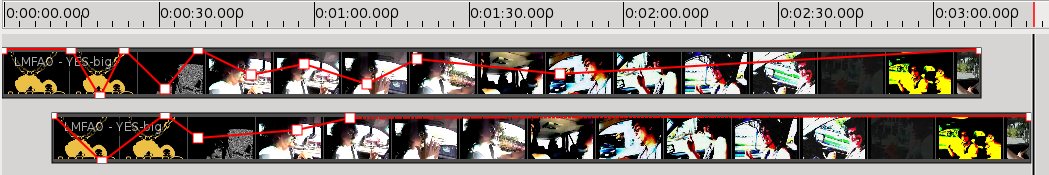
\includegraphics[width=0.9\textwidth]{images/keyframecurves}
  \end{center} \caption{Les keyframes} \label{Yes}
\end{figure}

\paragraph{}
Dans la création de clips en particulier, afin de dynamiser la vidéo,
les monteurs utilisent de manière intensive les keyframes.

\subsection{Fonctionnalités spécifiques}
%Ils  que dans %FIXME
%les fait, les fonctionnalités utilisés sont assez similaire bien que
%les œuvres finales soient totalement différentes.

\paragraph{}
Quelques fonctionnalités sont apparues comme vraiment propres à la création
d'un type d'oeuvre en particulier.

\subsubsection{Visualisation image par image:}
\paragraph{}
Dans le cadre de la création de film, la prévisualisation de chaque frame,
de manière précise semble être une fonctionnalité essentielle,
cela signifie, que le logiciel de montage doit permettre de
voir de manière simple chaque frame des vidéos présentes dans la
timeline. Cette fonctionnalité est aussi utile dans le cadre de
la création d'autres oeuvre, mais est indispensable dans le cadre
de film, afin de s'assurer de la qualité du résultat. En effet,
lors de la création d'un film, chaque frame doit être contrôlée,
alors que dans d'autres types d'oeuvre, les exigences étant moins
élevées ainsi que les moyens, une telle fonctionnalité ne est pas
indispensable.

\newpage
\begin{figure}
  \begin{center}
    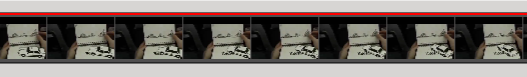
\includegraphics[width=0.9\textwidth]{images/frameByFrame}
  \end{center} \caption{Visualisation frame par frame} \label{Yes}
\end{figure}

\subsubsection{Gestion avancée des Footages}
\paragraph{}
Dans le cadre de productions longues, un des problème auquel doit répondre de
manière satisfaisante le logiciel d'édition est la gestion et la classification
des Footages. Cela est en particulier vrai pour les films et les séries télévisées.
Dans ces types de production le nombre d'heures de Footages peut être très grand, et
le monteur doit dans un premier temps, établir une classification
des Footages. Le logiciel de montage doit, pour répondre aux besoins des monteurs,
permettre de les ordonner de manière précise et bien pensée.

\subsubsection{Intégration dans un écosystème de logiciel de post production}
\paragraph{}
Dans le cadre de création de film en particulier, on constate qu'il est nécessaire
que le logiciel de montage puisse s'intégrer dans l'écosystème de logiciel de post
production. Cela est en général possible si ce logiciel de montage respecte les
quelques standard de la post production d'oeuvre audiovisuel comme par exemple le
Material eXchange Format \footnote{Material eXchange Format ou MXF est un conteneur
utilisé par les professionnels pour les données audio et vidéo numériques.
Il s'agit d'un format défini par des standards de la SMPTE. (Source: wikipedia)}

\subsubsection{Time remapping}
\paragraph{ }
Le time remapping, comme précédemment indiqué, est particulièrement utilisé dans
la création de contenu court. Il permet d'accélérer, où ralentir une partie d'un
clip pour le rendre l'œuvre la plus dynamique possible.

\subsubsection{Gestion des templates}
\paragraph{ }
La création de contenu non post produit demande des particulières. La fonctionnalité
qui apparaît comme clé pour répondre aux besoins liés à ce type de produit, est la
création de template. Par exemple, la création de journaux télévisés, ou autres évènements
sportifs (dans les faits presque tout ce qui est montage télévisé) demande une gestion avancée de ``moule``,
ou template, qui permet de simplement lier les contenus des différentes caméra 
à un moment donné de la retransmission.

\paragraph{ }
Cette fonctionnalité n'est pas exclusivement utilisée dans la création de contenu en direct, mais
elle est très largement utilisée dans tout ce qui est contenu destiné à la télévision.

\paragraph{}
\paragraph{}
En conclusion, on a constaté que le champ de fonctionnalité est vaste, la plupart de ces
fonctionnalités sont génériques et leur
utilisation est commune à différents types d'œuvres. Ce qui varie particulièrement  est
la finesse d'implémentation et le niveau d'utilisation qu'en fait le monteur.

\newpage
\section{Comparaison des principaux logiciels présent sur le marcher de
l'édition vidé professionnel, et analyse des manques et risques du marché}

\paragraph{}
  Il conviendra d'analyse en profondeur les logiciels existants, qu'il soit
  propriétaires ou libre. Cette partie à pour but de rendre compte de
  l'état actuel du marcher des logiciels d'édition vidéo qui on pour principal
  public les professionnelle de l'édition vidéo. Cette étude étant principalement portée
  sur le logiciel libre, ceux-ci seront évidemment inclus dans cette analyse
  bien que l'on puisse considérer que de par leur manque de maturité
  n'y ont pas totalement leur place. Dans cette optique, on se doit d'analyser
  différent points clé des logiciels qui peuvent être défini comme:

  \subsection{Fonctionnalités}
  \subsection{Prix}
  \subsection{Documentation}
  \subsection{Support}

\chapter{Analyse des opportunités des technologies libres dans le
domaine de l'édition vidéo et prévisions}

\minitoc \newpage

\paragraph{}

Maintenant que les besoins et que les solutions existantes ont été
analysées on rendra compte de la situation actuelle des technologies
libres et de leurs communautés. Il est aussi important de chercher les
raisons qui expliquent que ces logiciels ne sont pas utilisés par les
professionnels. Puis, nous essayerons d'envisager les solutions possibles
qui permettraient de remédier à cette situation.

\paragraph{}

Dans cette partie, nous analyserons la différence entre les manières
d'envisager la création de logiciel et nous verrons quels sont les
avantages et inconvénients de ces fonctionnements. Par la suite nous
nous concentrerons sur les frameworks existants pour faire une analyse
technique des ces technologies. Par la suite, nous analyserons les
communautés qui portent ces différents projets afin d'arriver à voir
les lacunes et les avantages de chacun des projets.  Pour finir, nous
tirerons les conclusions de cette analyse afin de trouver des solutions
aux défis qu'est la création d'un logiciel libre de montage vidéo.

\newpage

\section {Etat actuel de l'offre de logiciel libre}

Le schéma suivant permet de résumer facilement la situation:

\begin{figure} [h]
  \begin{center}
    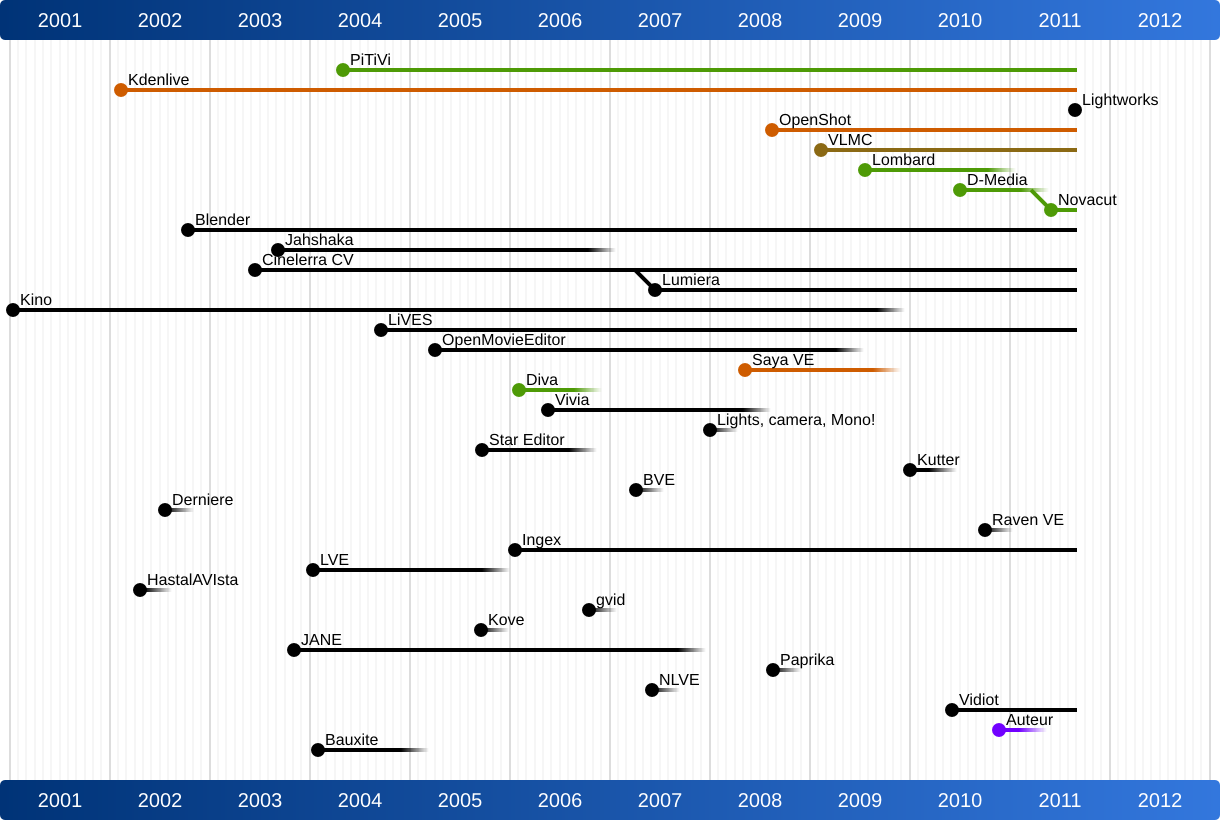
\includegraphics[width=0.9\textwidth]{images/open-source-video-editor-timeline}
  \end{center} \caption{Open source video editors timeline (Auteur:
  Jean-François Fortin, PiTiVi designer)} \label{Yes}
\end{figure}

\paragraph{ }

On constate donc que de nombreux projets de logiciel libre de montage
vidéo on vu le jours ces 10 dernières années, ayant différents
objectifs.  On peu distinguer deux types de publique visés par ces
projets:

\begin {itemize}

  \item {Les amateurs}

  \item {Les professionnels ou semi professionnels}
\end {itemize}

\paragraph {Les amateurs de montages vidéo}

\subparagraph{}

Plusieurs projets, libre permettent ou visent à répondre au besoins
des amateurs, mais à l'heure actuel même ce cas d'utilisation n'est
pas pleinement satisfait par les logiciels libres. Parmi les logiciels
ayant l'objectif de permettre de créer des montage simple on distingue:

\begin {itemize}

  \item {openshot: Logiciel avec de nombreuses fonctionnalité, mais don la
    qualité d'implémentation laisse à désirer.}

  \item {kino: Logiciel avec peu de fonctionnalité permettant de faire des
    petit montages éfficacement}

  \item {Vidiot qui vise la production de vidéo amateur simple}

\end {itemize}

\paragraph {}

Mais les logiciels ayant pour objectif de pouvoir aux besoins plus
avancés tel que ceux des professionnels (précédemment présenté
dans le cadre de la définition des plus grands acteur du marché)
peuvent être utiliser dans le cadre de montage amateur.

\paragraph{}

Un nouveau projet a aussi récemment vu le jours, ayant un but assez
différent des logiciel actuellement présent. Il s'agit de Novacut,
qui a pour but de permettre aux créateur de film et séries web de
faire le montage de manière collaborative à travers d'Internet, en
partageant les ressources (footage).

\paragraph{}

Cela montre qu'aucun projet n'a encore réussi à s'imposer et ainsi
regrouper les développeurs au sein de projets majeurs. Dans d'autre
domaine, cela a été le cas, par example dans le domaine des lecteurs
vidéo, Vlc a su surpassé ces concurrent, et ainsi supplanté le
marché des lecteur vidéo, qu'il soit libre ou non. Dans le domaine
des environnements de Bureau graphique, KDE et Gnome sont arrivés à un
stade ou leur supériorité technique, et en terme de fonctionnalités
fait d'eux des plateformes de référence.

\paragraph{}

Il est donc intéressant de se demander quel(s) technologie(s),
logiciel(s), pourrai(ent) se voir attribuer cette place dans le monde
de l'édition vidéo libre. Nous allons donc analyser les logiciel
et technologies libre les plus avancés, (précédemment mentionné
dans le cadre de l'analyse de marché: Cinelerra, Kdenlive et PiTiVi)
et ainsi voir si celui-ci, ou ceux-ci, ont le potentiel de pouvoir un
jours rivaliser avec les logiciels propriétaires sur le marché très
fermé du montage vidéo professionnels.

\paragraph{}

NB: Il aurait été intéressant d'analyser le logiciel lightworks,
en voix de libération, mais à l'heure actuel, aucun code n'a été
libéré, et par conséquent, celui-ci ne peut faire partit de cette
analyse.

\newpage

\section{Technologies}

\paragraph{}

Pour faire une analyse technique des produits permettant de faire
de l'édition vidéo, il est nécessaire d'analyser le ``core'' des
logiciels, c'est à dire la partie du logiciel où les opérations
d'édition sont effectivement réalisées. Dans ce domaines, il existe
deux façon de procéder:

\begin{itemize} \setlength{\itemsep}{2mm}

  \item{Création d'un logiciel monolithique\index{monolithique}}

  \item{Création d'un framework \glossary {name={framework},
   description={ Un framework est un ensemble d'outils et de composants
   logiciels organisés conformément à un plan d'architecture et des
   design patterns}} \index{framework}}

\end{itemize}

\subsection {Technologies monolithique\index{monolithique} VS technologies
modulaires, frameworks}


\subsubsection{Logiciels monolithiques \index{monolithique}} %FIXME Look
                                                             %for a def

\paragraph{}

Le conception monolithique \index{monolithique} dans le cadre des
logiciels d'édition vidéo, consiste à développer au sein d'un même
entité de code:

\begin{itemize} \setlength{\itemsep}{2mm}

  \item {la partie graphique et la partie de calculs
    permettant la gestion de tout ce que l'édition non linéaire
    implique}

  \item {L'interface utilisateur.}

\end {itemize}

\paragraph{}

Par le terme logiciel monolithique\index{monolithique}, il convient
de comprendre que le logiciel peut utiliser des librairies externes,
mais le core de ce même logiciel, et la logique d'édition linéaire
à proprement parler est directement faite à l'intérieur du logiciel
et non par une librairie où framework \index{framework} externe. Cela a
pour principal avantage que la conception est simplifiée pour plusieurs
raisons à savoir:

\paragraph{}

Les logiciels professionnels (commerciaux) utilisent très probablement
tous ce mode de fonctionnement (même si probablement, en interne il ont
un core qui ressemble fortement à un framework \index{framework}). Au
niveau des logiciels libres, le logiciel Cinelerra est un exemple
dans lequel les développeurs ont décidé d'utiliser ce mode de
fonctionnement.

On peu voir plusieurs conséquences immédiate de ce mode de
développement:

\begin{itemize} \setlength{\itemsep}{2mm}

  \item {Les développeurs n'ont pas la nécessité de penser
    en terme d'interface publique de programmation (API\index{API}), et
    n'ont pas à garantir la stabilité de celle-ci. Cela a pour effet que
    la qualité de l'architecture risque de ne pas être optimale puisque
    la création d'API\index{API} oblige les développeurs/architectes
    à réellement analyser les besoins de manière plus large dès le
    début de la conception. Dans le cas où l'on ne crée pas d'interface
    publique de programmation voué à être réutilisée, le risque est
    que le travail de design et d'architecture ne soit pas réalisé,
    et que le code grandisse de manière anarchique avec les différents
    développeurs qui ajoute leur morceau au fur qu'ils en ont besoin.}

  \item {Les développeurs n'ont besoin de penser l'architecture que pour
    les seuls cas d'utilisation qui sont liés à ce même logiciel,
    ils n'ont pas à voir au delà de ces use cases.}

  \item {Les erreurs en terme de design n'ont pas d'incidences aussi
    graves que dans le cas d'un framework\index{framework}.}
\end {itemize}

\paragraph{}

On se rend compte que cette manière de faire a pour principal avantage
le fait que le logiciel peut être développé plus rapidement puisque
le core du logiciel, et donc le code qui implémente la logique de
l'édition non linéaire est conçue avec pour seul cas d'utilisation,
celui du logiciel. Cependant, de nombreux inconvénients existent de
par la nature monolithique\index{monolithique} du design:

\subparagraph{Besoins en main d'oeuvre considérables:}

\subparagraph { }

Dans le cadre de logiciel d'édition vidéo, le code à produire est
considérable, comme le montre les statistiques (Annexes 2). Le logiciel
Cinelerra à lui seul fait plus d'un million de lignes. Une telle
quantité de code est difficile à maintenir et requiert des ressources
importantes en terme de main d'oeuvre. Le fait que le logiciel soit
monolithique\index{monolithique} implique que celui-ci va être utilisé
que par ce logiciel, et par conséquent, les développeurs ne peuvent
conté sur d'autre usage de ce code pour améliorer, développer le core
du logiciel.

\paragraph{Réutilisabilité:}

\subparagraph { }

L'un des inconvénients de cette manière de faire est que le code que
l'on a à l'intérieur du logiciel n'est pas réutilisable directement
par d'autres projets, et par conséquent, on peut considérer que cela
est ``individualiste``, chose qu'il convient d'éviter dans le cadre du
développement de logiciel libre afin de ne pas multiplier les efforts,
et dupliquer le code.

\paragraph{}

Cette façon de faire a été utilisée par le projet Cinelerra. Ce
logiciel est le plus avancé en terme de fonctionnalités que le
marché des logiciels libres de montage offre. On peut penser que son
architecture monolithique\index{monolithique} expliquer ce développement
plus abouti. Bien qu'il y ait évidemment de nombreux autre facteurs
tel que le fait que ce logiciel a été développé par la société
Heroine Virtual.

\subsubsection {Utilisation de  frameworks \index{framework}}

\paragraph{} L'autre possibilité est de séparer en deux parties logiciel
bien distincts l'implémentation de la logique de l'édition, lecture,
encoding vidéo (core logiciel), de la partie graphique, interaction
avec l'utilisateur final.

\paragraph {Le framework}

\subparagraph{}

La grande différence entre la conception monolithiques
\index{monolithique} et la création d'un framework \index{framework}
réside dans le le fait que dans le cadre d'un framework, on développe
une API \index{API} autour du core du logiciel. Cela résulte dans le
fait que le core est un programme (librairie) externe, réutilisable par
n'importe quel autre application.  On peut considérer que les avantages
des frameworks sont les inconvénients des applications monolithique
\index{monolithique} et vis versa. Le gros avantages des frameworks sur
une conception monolithique\index{monolithique} est la possibilité de
partager un même code à travers de multiple application. Celà permet de
réunir les efforts au travers, dans notre cas précis, de tout type d'application
multimedia.

Dans le cadre de l'édition vidéo, on peu encore distinguer deux manière
d'envisager son développement:

\begin {itemize}

  \item {Utiliser un framework multimedia généraliste, et créer les
  outils nécessaire
         au montage au dessus de celui-ci} %stupid french!\ldots On top
                                           %of it?

  \item {Créer un framework spécialement orienté montage vidéo}

\end {itemize}

Dans le monde du logiciel libre, ces deux manière d'envisager le
développement d'un framework multimedia ont été abordé par les deux
projets de framework leader sur ce segment:

\begin {itemize}

  \item {MLT qui se défini comme étant un ``Framework multimedia design
    et développé pour le brodcasting télévisé.''}

  \item {Gstreamer qui se défini comme étant un ``framework multimédia
    basé sur la notion de pipeline ce qui lui permet de nombreux types
    d'applications multimedia tel que des lecteurs multimédia, des
    logiciels de broadcasting, des logiciel de montage vidéo\ldots''}

\end {itemize}

\subparagraph {}

Au dessus de ces frameworks, deux application (interfaces graphique)
de montage vidéo se sont développé.

\begin {itemize}

  \item {PiTiVi: utilise le Framework multimedia GStreamer}

  \item {Kdenlive utilise le framework\index{framework} orienté édition et
    broadcasting MLT.}

\end {itemize}

\paragraph {}

Dans le cadre des Frameworks, nous nous intéresserons
en particulier à l'analyse de ceux-ci puisque les notions relatives
à l'édition vidéo, et la gestion de toute la partie multimédia est
réalisée par ceux-ci. Les logiciels d'édition ne sont à priori que
de simples interfaces graphiques basées sur ces frameworks, et par
conséquent leur analyse ne présente qu'un faible intérêt.

\newpage \section{Analyse technique}

\paragraph {}

Dans cette partie nous allons analyser les entrailles des trois logiciels précédemment
définis: Cinelerra, PiTiVi et Kdenlive.

\subsection{Cinelerra:}

\paragraph {}

Cinelerra est le logiciel d'édition audio et vidéo et de composition le plus
avancé dans le monde de logiciel libre. Il est développé principalement par
Adam Williams pour l'entreprise Heroine Virtual Ltd. Ce projet a été initié
en 2001 sous le nom de broadcast2000 par cette même entreprise.

\paragraph{}

Le logiciel Cinelerra a été développer principalement en C++ et est composé de 3 partie
principal interdépendantes:

\begin{itemize}

  \item{Lecture/et rendering audio vidéo}

  \item{Edition vidéo non-linéaire}

  \item{Interface graphique}

\end{itemize}

\subsubsection{Lecture et rendering}

\paragraph{}

Dans le cadre de la lecture audio et video, Cinelerra fait appelle à diverse library:

\begin{itemize}

  \item{ffmpeg: Solution compete, cross plateforme d'enregistrement, lecture, conversion
    de flux audio et vidéo. Il inclus libavcodec, librairie leader dans le domaines des codec.
    Il s'agit du core de la lecture audio et vidéo de Cinelerra.}

  \item{faac/faad: AAC audio encoder}

  \item{x264: h264 encoder}

  \item{x264: h264 encoder}

  \item{\ldots}

\end{itemize}

\subparagraph{}

Toutes ces librairies sont utilisé dans le but de lire et écrire des fichiers multimedia.
Afin de standardizer, et permettre l'utilisation de ces libraries de manière similaire
au sein du logiciel, les développeur de Cinelerra ont développé au cas par cas des pont entre
ces librairies et le reste du logiciel (Fichier dans le dossier quicktime).

\paragraph{Edition non linéaire}


\newpage \section{Analyse des communauté}

\newpage \section{Lacunes}

\newpage \section{Solutions possibles}


\section{Conclusion}

\newpage
\tableofcontents
\listoffigures

\newpage
\newpage

\chapter*{Annexes}
\section*{Interview de Sophian Veri,
Responsable Post Production chez Be Movie, France}

\paragraph{}
1-  Quelles logicielles d'éditions vidéos utilisez-vous à l'heure actuelle?

Sophian Veri: J'utilise exclusivement finalcut.

\paragraph{}
2- Quels formats de vidéos produisez vous?

Sophian Veri: Je produis des clips, reportages, pubs et courts métrages.

\paragraph{}
3- Ce logiciel répond-t-il à tous vos besoins en terme de montage?
Sophian Veri: généralement oui.

\paragraph{}
4- Quels défauts vous viennent à l'esprit quand vous pensez à cette outil?

Sophian Veri: le montage multicamera est mal géré, le temps de rendu trop long car le
logiciel ne fonctionne pas avec toute la mémoire vive de l'ordinateur
contrairement à la suite Adobe.

\paragraph{}
5- Considérez-vous Final Cut Pro comme étant la meilleure solution de montage,
si oui, pourquoi?

Sophian Veri: Oui, sans aucun doute. Pour sa facilité d'utilisation,
les codecs acceptés y sont nombreux et la liste des effets est
longue\ldots

\paragraph{}
6-  Quelles fonctionnalités utilisez vous au quotidien (ex: Multicamera, effets,
transitions, keyframes, time remapping, outils collaboratifs, proxy
editing, Templates...)

Sophian Veri: effets de mauvais téléviseur, time remap, cache patate (qui m'évite
de passer par after.) ralenti, fondu enchainé.

Thibault Saunier: Qu'est-ce que cache patate?
Sophian Veri: cache patate, c'est masque dans after.

\paragraph{}
7-  Quelles fonctionnalités considérez-vous comme indispensables, (même si vous
ne les utilisez pas au quotidien)?

Sophian Veri: la modification des couleurs,  tout ce qui est travail de
l'image, contraste, netteté, saturation.

\paragraph{}
8- Quel pourcentage de fonctionnalités du logiciel pensez-vous utiliser
en tout?

Sophian Veri: il y a  tellement de fonctionnalités que je serais tenté
de dire 25\%.

\paragraph{}
9- Seriez vous prêt à utiliser des logiciels ayant moins de fonctionnalités,
mais qui répondraient de manière plus efficace à vos besoins?

Sophian Veri: pourquoi pas à condition qu'ils soient aussi intuitifs et que les effets
que j'utilise soient tout aussi bien gérés.

\paragraph{}
10-  Le prix du logiciel est-il un critère de choix selon vous?

Sophian Veri: oui, en tant que nouvelle jeune entreprise, le prix est
un critère de choix.

\paragraph{}
11- Avez-vous des problèmes de stabilité (de bugs) avec finalcut?

Sophian Veri: les bugs, assez rarement.

\paragraph{}
12- La dépendance vis-à-vis du créateur du logiciel que vous utilisez
vous parait-elle être quelque chose de dangereux?

Sophian Veri: oui dans le sens où on ne sait jamais quelles transformations le
logiciel subira avec la version suivante. Il arrive que la version soit moins adaptés
et qu'elle ne me donne plus toute satisfaction. C'est le cas il me semble de Final Cut
X qui a l'air d'être raté.

\paragraph{}
13- Connaissez-vous certains logiciels libres d'édition vidéo?

Sophian Veri: Je ne sais pas vraiment ce que c'est.

Thibault Saunier: Merci bien d'avoir pris le temps de répondre

\newpage\section*{Interview de Karim Hachemi, Monteur chez Falfyprod, Film d'entreprise,
Court Métrages et film de mariage, France}

\paragraph{}
1-  Quel logiciel d'édition vidéo utilisez vous à l'heure actuel?

Karim Hachemi: Final cut mais surtout Adobe CS5.

\paragraph{}
2- Quel types de vidéo produisez vous?

Karim Hachemi: Clips, Pubs et institutionnels.

\paragraph{}
3- Ce logiciel répond-t-il à tous vos besoins en terme de montage?

Karim Hachemi: Adobe Première non, mais Final Cut oui.
Nous somme obligé d'utiliser Adobe première du fait que
le format produit par la camera Canon 5D est mal supporté par Final Cut.
Nous aurions donc besoin de les convertir et nous perderions beaucoup de
temps, c'est pourquoi nous utilisons la suite adobe bien qu'elle ne nous donne
pas complètement satisfaction.

\paragraph{}

4- Quels défauts vous viennent à l'esprit quand vous pensez à cet outil?

Karim Hachemi: Final cut est un tout petit peu plus compliqué mais
est plus complet.


\paragraph{}
5-  Quels fonctionnalités utilisez-vous au quotidien (ex: Multicamera, effets,
transitions, keyframes, time remapping, outils collaboratifs, proxy
editing, Templates...)

Karim Hachemi: Effets et transitions, en général je me sers que de ça.

\paragraph{}
6-  Quelles fonctionnalités Considérez-vous comme indispensables, (même si vous
ne les utilisez pas au quotidien)?

Karim Hachemi: le rognage de final cut sur première est mal conçu et c'est très
énervant.

\paragraph{}
7 Quel pourcentage des fonctionnalités du logiciel pensez-vous utiliser
en tout?

Karim Hachemi: Je dirais 30-35%

\paragraph{}
8- Seriez-vous prêt à utilisez des logiciels ayant moins de fonctionnalités,
mais qui répondraient de manière plus efficace à vos besoins?

Karim Hachemi: cela dépend s'il manque des fonctionnalités dont je ne me
suis jamais servi cela m'est égal.

\paragraph{}
9-  Le prix du logiciel est-il un critère de choix selon vous?

Karim Hachemi: oui.

\paragraph{}
10- Avez-vous des problèmes de stabilité (de bugs)?

Karim Hachemi: non pas trop de bugs mais ce qui est ennuyeux c'est les
rendus beaucoup trop long.

\paragraph{}
11- Connaissez-vous certains logiciels libre d'édition vidéo?

Karim Hachemi: Non, mais il faut que j'essaie.

\newpage\section*{Interview de Yves Faure, responsable technique chez TL7
(Télévision de Saint Étienne)}

\paragraph{}
1-  Quel logiciel d'édition vidéo utilisez-vous à l'heure actuelle ?

Yves Faure: Pour le montage video, j'utilise principalement Final cut pro. Il
arrive dans de très rares cas que l'on utilise adobe premiere. Notre
parc informatique est basé sur mac. En ce qui concerne l'habillage et
l'infographie on utilise ``photoshop'' et  ``After Effect'' pour les effets (bien
que dans de nombreux cas, on fasse les effets directement dans Final Cut).

\paragraph{}
2- Quel format de vidéo produisez-vous?

Yves Faure: Un peu de tout: Reportages, documentaires, plateaux magazines, films de reportage, spots
publicitaires, captations musique et théâtral.

\paragraph{}
3- Ce logiciel répond-t-il à tout vos besoins en terme de montage?

Yves Faure: Oui, largement. Nous avons des besoins spécifiques en terme d'organisation,
archivage, gestion de sous-titrage, mais cela sort du scope du logiciel de
montage.

\paragraph{}
4- Quels défauts vous viennent à l'esprit quand vous pensez à cet outil?

Yves Faure: Le problème important qui me vient à l'esprit est le fait que Final Cut 10 soit
extrêmement osé. Apple a décidé de revoir complètement l'interaction
utilisateur et cela va nous faire perdre du temps (et donc de l'argent).

Il y a aussi de petits défauts d'ergonomie qui sont irritants.

Le fait qu'il soit aussi puissant est pour nous un défaut puisque cela
complexifie la tâche du monteur.

Son prix très élevé est aussi un problème pour notre structure (bien que bien
moins cher que d'autres concurrents).

Par défaut, les fichiers de rendu video, le cache de vignette, est stocké dans
le dossier final cut pro global au  système et pas avec le projet, ce qui
signifie que l'on doit changer cela à chaque fois et une fois de plus c'est une
perte de temps importante.

Lorsqu'il y a des ruptures de timecodes dans les fichiers, le logiciel réagit mal
et cela est régulièrement une source de problème.

La gestion des formats est assez mauvaise.

Trop configurable en tout points.

Pas de sortie moniteur directe chez Apple. Pour visualiser le rendu final sur les
moniteurs et ainsi être sur de la qualité du montage (en particulier au niveau de
la lumière et des couleurs, on est obligé d'effectuer le rendu et ensuite
seulement le voir sur les moniteurs dédiés. On devrait pouvoir brancher nos Mac
sur les moniteurs et regarder en temps réel le résultat final.

\paragraph{}
5- Quelles sont les qualités apportées par ce logiciel et qui vous donne satisfaction?

Yves Faure: La dernière version de Final cut permet le réetalonage automatique (de l'image
et du son), cela va vraiment faciliter le travail des monteurs.

Le fait qu'il s'agit du standard actuel dans le milieu est très important pour
nous. Cela nous permet de communiquer facilement avec nos confrères.

Le fait aussi que l'on ait les effets directement intégrés dans le logiciel nous
permet d'accélérer le montage dans de nombreux cas.

Dans le cadre de magazines et films publicitaires, on utilise beaucoup les
animations (transformations) tel que la modification de l'échelle de l'image,
le rognage. Aussi, le lissage des bords et les ombres portés de l'image nous
permettent régulièrement de faire des montages mieux léchés.


\paragraph{}
6- Pour vous, finalcut est la meilleure solution de montage?

Yves Faure: Oui, c'est sûr.

\paragraph{}
7-  Quelles fonctionnalités utilisez-vous au quotidien (ex: Multicamera, effets,
transitions, keyframes, time remapping, outils collaboratifs, proxy
editing, Templates...)

Yves Faure: Au quotidien, nous utilisons: Transition, effet, mixage audio, montage cut,
retouche de couleurs, étalonnage, colorimétrie, multi-images, gestion de la
vitesse par clip entier, pas de time remapping à proprement parlé.

\paragraph{}
8-  Quelles fonctionnalités considérez-vous comme indispensables, (même si vous
ne les utilisez pas au quotidien)?

Yves Faure: Je pense que le multicamera (pour la couverture d'évènement tel que les
concerts) est la fonctionnalité importante, même si elle n'est pas utilisée au quotidien.

\paragraph{}
9- Quel pourcentage des fonctionnalités du logiciel pensez-vous utiliser
en tout?

Yves Faure: En général 10\%, jusqu'à 50\% maximum.

\paragraph{}
10- Seriez-vous prêt à utiliser des logiciels ayant moins de
fonctionnalités, mais qui répondrait de manière plus efficace
à vos besoins?

Yves Faure: Non, car nous sommes très attachés à la connaissance du logiciel.
Changer de logiciel signifie 40 personnes à former, changer les
habitudes et cela est très complexe en particulier pour les professionnels
du montage vidéo! Nous avons une solution qui nous convient et qui est leader
sur le marché, il faudrait une vrai évolution du marché pour que l'on pense à
changer.

\paragraph{}
11-  Le prix du logiciel est-il un critère de choix selon vous?

Yves Faure: Oui et non, c'est cher mais ça marche. Autant se donner les moyens pour avoir
un produit qui nous permet de gagner par la suite.

\paragraph{}
12- Avez-vous des problèmes de stabilité (de bugs) avec Final Cut?

Yves Faure: Non, la stabilité est un point fort de Final Cut.

\paragraph{}
13- La dépendance vis-à-vis du créateur du logiciel que vous utilisez
vous paraît-elle être quelque chose de dangereux ?

Yves Faure: Non, on s'arrange comme on peut. La version que l'on utilise actuellement
nous convient. S'il faut continuer avec celle-ci, on le fera.


\newpage
\bibliography{biblio}

\end{document}
